\documentclass[11pt,a4paper]{article}
\usepackage[margin=21mm,top=21mm,bottom=21mm]{geometry}
\usepackage[T1]{fontenc}
\usepackage{lmodern,microtype,amsmath,amssymb,booktabs,tabularx,array,graphicx,caption,xcolor,fancyhdr,tikz,enumitem}
\usetikzlibrary{positioning,arrows.meta,shapes.geometric}
\usepackage[numbers,sort&compress]{natbib}
\usepackage[hidelinks]{hyperref}
\definecolor{navy}{HTML}{173650}
\definecolor{teal}{HTML}{237C76}
\definecolor{light}{HTML}{EAF1F3}
\setlength{\parindent}{0pt}
\setlength{\parskip}{5pt plus 1pt minus 1pt}
\setlength{\headheight}{14pt}
\setlength{\tabcolsep}{5pt}
\renewcommand{\arraystretch}{1.14}
\setlist{nosep,leftmargin=*}
\captionsetup{font=small,labelfont=bf,skip=4pt}
\pagestyle{fancy}\fancyhf{}\fancyhead[L]{\small\textcolor{navy}{EDA Assistant | Research report}}\fancyhead[R]{\small November 2026}\fancyfoot[R]{\small\thepage}\renewcommand{\headrulewidth}{0.4pt}
\newcommand{\code}[1]{\texttt{#1}}
\newcommand{\pairfig}[4]{\begin{center}\begin{minipage}[t]{.49\linewidth}\centering\includegraphics[width=\linewidth]{figures/#1}\captionof{figure}{#2}\end{minipage}\hfill\begin{minipage}[t]{.49\linewidth}\centering\includegraphics[width=\linewidth]{figures/#3}\captionof{figure}{#4}\end{minipage}\end{center}}
\newcommand{\widefig}[3]{\begin{center}\includegraphics[width=#1\linewidth]{figures/#2}\captionof{figure}{#3}\end{center}}
\newcommand{\tbl}[1]{\captionof{table}{#1}}
\begin{document}
\thispagestyle{plain}
\begin{center}
{\small\bfseries\textcolor{teal}{PROJECT RESEARCH REPORT}}\\[8pt]
{\LARGE\bfseries\textcolor{navy}{Evidence-Grounded LLM Framework for\\ Intelligent EDA Log Analysis}}\\[6pt]
{\large A comparative study of direct prompting, lexical RAG and hybrid structured retrieval}\\[9pt]
{\small 24 November 2026}
\end{center}
\vspace{2pt}\hrule\vspace{5pt}
\begin{abstract}
Electronic design automation (EDA) tools generate many logs containing timing, power, area and execution information. Finding answers in these files can be difficult, especially when a question involves several reports. In this project, we use NVIDIA's EDAFlowQA benchmark to compare three methods: Direct prompting with limited raw log context, Standard retrieval-augmented generation (RAG) using BM25, and Hybrid RAG using both logs and structured metrics. We also implemented a Python calculator for Hybrid. We tested Qwen3-4B locally on 40 questions across three designs, giving 120 attempts in total. Direct, RAG and Hybrid achieved full-answer accuracies of 2.5\%, 7.5\% and 17.5\%, respectively. Hybrid used more tokens and took longer than RAG. In an earlier, incomplete GPT-OSS-20B experiment on Groq, Hybrid was again the most accurate, but used fewer tokens and responded faster. Neither run recorded a successful calculator trace or a fully correct answer in the two complex question categories. These results show where structured retrieval helps and where the system still needs improvement.
\end{abstract}
\textbf{Keywords:} electronic design automation, EDAFlowQA, BM25, retrieval-augmented generation, structured metrics, question answering.

\section{Introduction}
A digital chip goes through several stages before the design flow is complete. These include synthesis, floorplanning, placement, clock tree synthesis, routing and final reporting. Each stage generates files that engineers use to check the progress of the design and identify problems. Finding a particular value can take time, especially if similar metrics are reported at different stages or if a question requires comparing numbers from several files.

We wanted to see whether an LLM could make this process easier by allowing users to ask questions in natural language. A model given raw text may read the wrong row of a table or confuse two stages. Retrieving relevant excerpts can reduce the amount of text it has to read, while structured measurements may make specific values easier to find. Even then, a valid citation does not necessarily mean the answer is correct.

\subsection{Research objectives}
Our main objective was to find out whether using structured metrics together with log retrieval would improve answer accuracy within a limited context size. We also wanted to study how well the methods handle numerical questions, provide sources and use computational resources. We deliberately kept the scope on the software side: we work with existing reports instead of generating RTL, running OpenROAD or modifying a chip. No model training or fine-tuning was needed, and the system does not perform physical-design signoff.

\textbf{Our contribution.} We built three QA methods, a validated calculator, an evaluator that records unsuccessful attempts, and a Streamlit interface for questions and saved results. The original benchmark and design measurements come from EDAFlowQA.
\newpage
\section{Related Work and Benchmark}
\subsection{Literature review}
We began by looking at how LLMs have been used in chip design. The LLM4EDA survey \cite{llm4eda} discusses assistants, HDL and script generation, and verification. We chose to work on the analysis side. EDAFlowQA \cite{edaflowqa,edadata} is particularly relevant because it focuses on reasoning over logs from different design stages. The authors extract OpenROAD metrics, generate questions using Q-Tree sampling and evaluate answers with Pass@K. We use their released data and questions but implement our own QA pipeline.

Retrieval-augmented generation (RAG) gives an LLM relevant external information before it answers a question \cite{lewis}. We chose BM25 \cite{bm25} for retrieval because it is simple to use and does not require training an embedding model. Pu et al. \cite{rageda} use semantic retrieval and a trained reranker for EDA tool documentation. Our work differs in that we search actual design logs and structured metric records using lexical retrieval, rather than combining dense and sparse search. TAT-QA \cite{tatqa}, a benchmark in finance, also uses tables and text for numerical questions. The idea of separating the retrieval of values from the actual calculation was useful for designing our calculator.
\subsection{Dataset and design scope}
EDAFlowQA contains 1,136 question-answer pairs, of which 909 concern individual designs and 227 compare designs. We selected three individual design runs and used repository revision \code{d1e43c6}, with the full revision saved in our configuration. The logs and reports are in \code{design\_artifacts/}, structured metrics in \code{extracted\_design\_stage\_metrics/}, and questions in \code{qa\_release/}. We retained the original Apache 2.0 license.
\begin{center}\small
\tbl{Indexed subset of official benchmark artifacts.}
\begin{tabular}{@{}lrrrrr@{}}\toprule
Design & Files & Lines & Chunks & Metrics & Released QA\\\midrule
\code{aes\_asap7} &10&7,120&397&574&80\\
\code{aes\_nangate45}&10&5,995&338&777&74\\
\code{ibex\_sky130hd}&11&8,969&503&818&73\\\midrule
Total&31&22,084&1,238&2,169&227\\\bottomrule
\end{tabular}\end{center}
The selected AES and Ibex runs use the ASAP7, Nangate45 and Sky130HD technology platforms. The indexed raw files occupy 1,715,385 bytes. Some lines appear in more than one chunk because of overlap. We use these runs as sources for questions, not to compare the quality of the technology platforms.
\subsection{Question selection}
We used random seed 42, shuffled questions by category and selected them in round-robin order. We removed identical normalized questions and near-duplicates with a \code{SequenceMatcher} similarity of 0.85 or more. Of the 40 selected questions, 17 are from AES ASAP7, 10 from AES Nangate45 and 13 from Ibex. They belong to 27 design-specific ID families, so some questions are related. We saved the selected IDs in the configuration to allow the same experiment to be repeated.
\begin{center}\small
\tbl{Question categories and their reasoning requirements.}
\begin{tabularx}{\linewidth}{@{}l r X@{}}\toprule
Category & Count & Task\\\midrule
Flow execution&9&Determine run status, errors or stages.\\
Single stage&11&Locate a metric or fact at a specified stage.\\
Multi stage&10&Compare measurements across stages.\\
Stage to final&10&Relate intermediate behavior to final results.\\\bottomrule
\end{tabularx}\end{center}
\newpage
\section{Methodology: Direct and Standard RAG}
\subsection{Problem formulation}
For a given question $q$ about design $d$, we define $L_d$ as the collection of raw logs and reports, and $M_d$ as the official structured metrics. The difference between our three methods is how they construct the evidence set $E_m(q,d)$. All of them pass this evidence to the same model $F_\theta$, which returns an answer $\hat a$ and a set of evidence IDs $C$:
\begin{equation}
(\hat a,C)=F_\theta(q,E_m(q,d)),\qquad |\operatorname{render}(E_m)|\le B.
\end{equation}
In our completed local experiment, $B=6{,}000$ characters. We keep the reference answers separate from the information sent to the model and use them only when scoring predictions. Answers that do not meet the validation rules can be rejected or flagged. All three local methods use the same model and generation settings.
\subsection{Method A: Direct LLM}
For the Direct method, we give the model a fixed sample of raw text for each design, regardless of the question. We select the main log and one representative report from each numbered stage group. Around 40\% of the available space is used for the main log and the rest is shared among the reports. We take excerpts from the beginning and end of the files and preserve their names and line numbers.

The resulting context sizes for the three designs are 4,973, 5,344 and 5,430 characters. This approach does not pass all the available logs to the model, so we refer to it as \emph{truncated direct prompting}. An important limitation of this baseline is that the required information may be in the original files but not in the selected excerpts.
\subsection{Method B: Standard BM25 RAG}
We first divide the raw logs into chunks of 24 lines, with an overlap of six lines, giving a stride of 18. Each chunk retains its filename and line range. Before indexing, we convert text to lowercase, split identifiers, remove common words and normalize some word variants. Filenames are also indexed, as they often contain stage names. For some count questions, we add the word \emph{total} to the query.

For a question with terms $t\in q$ and a log chunk $x$, BM25 calculates the relevance score as follows \cite{bm25}:
\begin{equation}
S(q,x)=\sum_{t\in q}\operatorname{IDF}(t)\,
\frac{f(t,x)(k_1+1)}{f(t,x)+k_1(1-b+b|x|/\overline{|x|})},
\end{equation}
Here, $f(t,x)$ is the frequency of a term in the chunk, $|x|$ is the chunk length, and $\overline{|x|}$ is the average chunk length. The parameters $k_1$ and $b$ control term-frequency saturation and length normalization. A common expression for inverse document frequency is
\begin{equation}
\operatorname{IDF}(t)=\ln\frac{N-n_t+0.5}{n_t+0.5},
\end{equation}
where $N$ is the total number of indexed chunks and $n_t$ is the number containing $t$. We use the \code{rank-bm25} library, which also handles negative IDF values. We did not tune these parameters separately.

We request eight ranked chunks, initially limiting the selection to two per source, with a fallback if needed. The evidence is fitted into the total character budget, with each log excerpt limited to 1,600 characters. The LLM then answers the question and cites the excerpts it uses. The overlap helps when information is near a chunk boundary, but it is still possible to separate a table header from its total row. BM25 can also retrieve the right metric from the wrong design stage.
\newpage
\section{Proposed Hybrid RAG Framework}
For Hybrid RAG, we keep the BM25 index of raw logs and add a second index for the individual values in the aggregate metric JSON files. Each structured record includes the design, stage, metric name, value, unit, source file and JSON path. The path lets us locate the original JSON field, although it does not always point back to a specific line in the raw log.

We retrieve up to 12 structured metric records and five raw chunks. Initially, 58\% of the available characters are allocated to the metrics, and the remaining space is used for the logs. Our idea is to give the model direct access to numbers while still providing the surrounding information, such as warnings and commands. There is also a drawback: long JSON paths and additional instructions can make the input more difficult to interpret.
\begin{center}
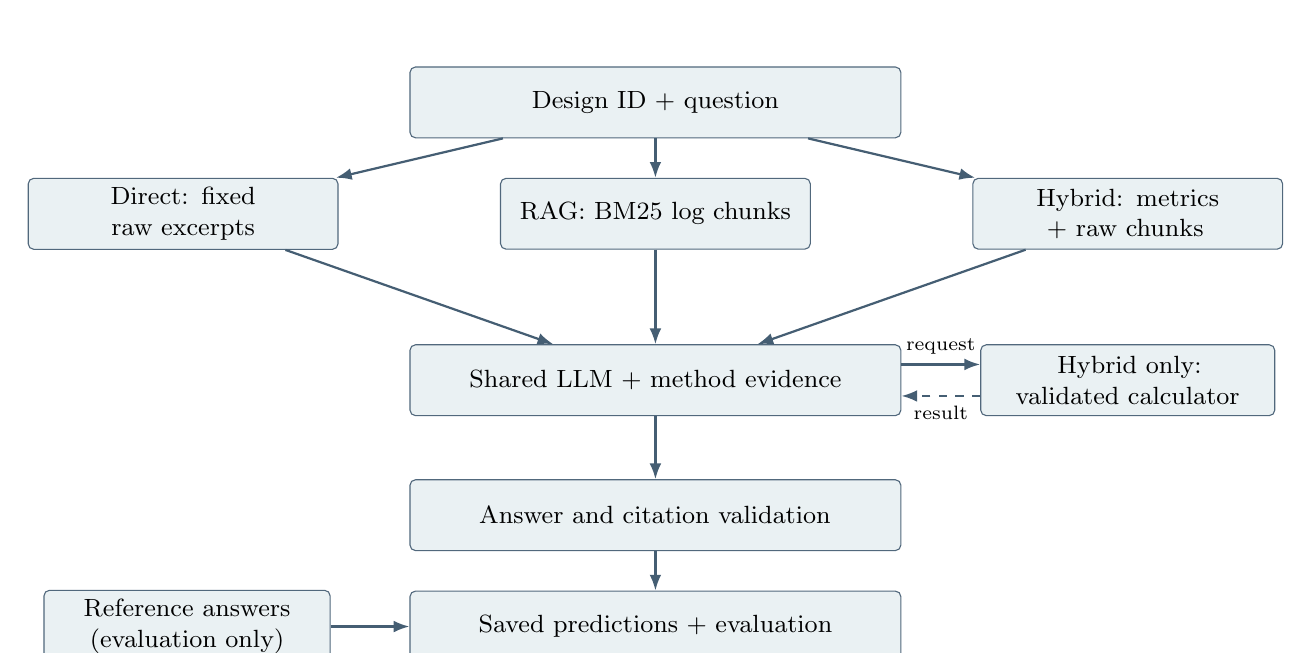
\begin{tikzpicture}[font=\small, node distance=5mm and 9mm, box/.style={draw=navy!75,rounded corners=2pt,fill=light,align=center,minimum height=9mm,text width=42mm}, narrow/.style={box,text width=37mm}, arrow/.style={-{Latex[length=2mm]},draw=navy!80,thick}]
\node[box,text width=60mm] (q) {Design ID + question};
\node[narrow,below left=of q] (d) {Direct: fixed raw excerpts};
\node[narrow,below=of q] (r) {RAG: BM25 log chunks};
\node[narrow,below right=of q] (h) {Hybrid: metrics + raw chunks};
\node[box,text width=60mm,below=12mm of r] (llm) {Shared LLM + method evidence};
\node[box,right=10mm of llm,text width=35mm] (calc) {Hybrid only:\\validated calculator};
\node[box,text width=60mm,below=8mm of llm] (v) {Answer and citation validation};
\node[box,below=of v,text width=60mm] (s) {Saved predictions + evaluation};
\node[box,left=10mm of s,text width=34mm] (ref) {Reference answers\\(evaluation only)};
\draw[arrow] (q)--(d);\draw[arrow] (q)--(r);\draw[arrow] (q)--(h);
\draw[arrow] (d)--(llm);\draw[arrow] (r)--(llm);\draw[arrow] (h)--(llm);
\draw[arrow] (llm)--(v);\draw[arrow] ([yshift=2mm]llm.east) -- node[above,font=\scriptsize]{request} ([yshift=2mm]calc.west);
\draw[arrow,dashed] ([yshift=-2mm]calc.west) -- node[below,font=\scriptsize]{result} ([yshift=-2mm]llm.east);
\draw[arrow] (v)--(s);\draw[arrow] (ref)--(s);
\end{tikzpicture}
\captionof{figure}{Implemented evidence flow. The conditional calculator result is supplied to a second LLM call before final validation.}
\end{center}
\subsection{Restricted numerical reasoning}
When a question involves arithmetic, the model can request a calculation using the IDs of numeric metrics that are present in its context. If $a$ and $b$ are the selected values, with $b$ as the baseline, the supported operations are
\begin{align}
\operatorname{difference}(a,b)&=a-b, & \operatorname{ratio}(a,b)&=a/b,\\
\operatorname{percentage\_change}(a,b)&=100(a-b)/|b|,\\
\operatorname{minimum}(\mathbf{x})&=\min_i x_i, & \operatorname{maximum}(\mathbf{x})&=\max_i x_i.
\end{align}
The calculator checks that the IDs are known and distinct, the values are numeric and finite, and the unit strings agree. It also rejects division by zero. Operations on two values require exactly two operands, while minimum and maximum accept between 2 and 12. When a calculation succeeds, the system saves the IDs, values, result and unit. The result can then be passed back to the LLM for a second call, and the final answer is checked against the computed value and the evidence IDs. For example, $0.156-0.113=0.043$ W illustrates a supported operation; this is not an actual benchmark calculation. At present, the calculator cannot extract numbers from raw tables or convert units on its own. Although we implemented and tested this component, neither experiment produced a successful calculation trace. We therefore cannot measure its effect on accuracy from these results.
\newpage
\section{Implementation and Experimental Protocol}
\subsection{Model configurations}
We initially used GPT-OSS-20B through the Groq API \cite{groq}. Later, we moved to a local Qwen3-4B model \cite{qwen} running through Ollama \cite{ollama}, using native JSON output and disabling thinking mode. We changed several settings during this migration, as shown below. For this reason, the two runs are not a controlled comparison of hosting providers.
\begin{center}\small
\tbl{Generation settings recorded in project documentation.}
\begin{tabularx}{\linewidth}{@{}lXX@{}}\toprule
Setting&Completed local run&Archived Groq run\\\midrule
Model&\code{qwen3:4b}&\code{openai/gpt-oss-20b}\\
Temperature&0&0\\
Evidence cap&6,000 characters&3,500 characters\\
Output cap&768 tokens&512 tokens\\
Context window&8,192 tokens&Not recorded\\
Reasoning&Thinking disabled&Low reasoning effort\\
Protocol&Version 8&Earlier, no version saved\\
Attempted per method&40 of 40&22 of 40\\\bottomrule
\end{tabularx}\end{center}
\subsection{Evaluation and metrics}
Our scorer checks normalized exact matches, numerical values with unit conversion (1\% relative tolerance plus small unit-specific absolute tolerances), equivalent structures and simple prose answers. Every requested field must match. Unclear cases are flagged for review. A bare number is interpreted in the reference unit. These rules differ from the original EDAFlowQA evaluator and may reject equivalent answers.

We evaluate $N=40$ selected questions. Let $c_i$ be 1 when the entire answer is correct and 0 otherwise, and let $I_{\rm num}$ represent the 36 questions whose references contain numerical information. We calculate the two accuracy measures as follows:
\begin{equation}
\mathrm{Pass@1}=\frac{\sum_{i=1}^{N}c_i}{N},\qquad
A_{\rm num}=\frac{\sum_{i\in I_{\rm num}}c_i}{|I_{\rm num}|}.
\end{equation}
Answer coverage is the proportion of questions with a retained answer. We also use $N$ as the denominator for abstentions, failures and valid citations. Questions that were not attempted add no correct answers. A valid citation only tells us that the cited ID was present in the context; it does not establish that the answer is supported by it. Mean response time excludes API failures but includes abstentions, retrieval and potentially index construction. Token counts are the saved input and output counters, rather than a complete measure of computational cost.
\subsection{Software and verification}
We used Python, \code{httpx}, \code{rank-bm25}, Pandas, NumPy, Matplotlib and Streamlit. Separate modules handle data, retrieval, inference, validation, arithmetic and evaluation. The runner saves each attempt in JSONL, resumes by design, question and method, checks configuration consistency and continues after individual generation failures. The Streamlit app has tabs for asking questions and viewing results.

The project documentation records nine passing offline tests, including a controlled-client test of the calculator's two-call workflow, and a Streamlit rendering check. Test responses are not benchmark predictions. This report uses the saved results and documentation, without rerunning inference or tests.
\newpage
\section{Results: Completed Local Experiment}
We completed all 120 attempts in the local experiment, with 40 questions for each of the three methods. One Direct request failed. The other attempts either returned an answer or abstained. Table~\ref{tab:local} shows the results using our original scoring rules.
\begin{center}\small
\tbl{Local Qwen3-4B results, fixed 40-question denominator.}\label{tab:local}
\begin{tabularx}{.95\linewidth}{@{}Xrrr@{}}\toprule
Measurement&Direct&Standard RAG&Hybrid RAG\\\midrule
Attempted questions&40&40&40\\
Correct answers&1&3&7\\
Overall accuracy&2.50\%&7.50\%&\textbf{17.50\%}\\
Numeric-reference correctness&0/36&2/36&6/36\\
Numerical accuracy&0.00\%&5.56\%&\textbf{16.67\%}\\
Retained answers&20&34&33\\
Answer coverage&50.00\%&85.00\%&82.50\%\\
Abstentions&19&6&7\\
API failures&1&0&0\\
Valid citations&18&32&31\\
Flagged for review&17&28&24\\
Mean response time (s)&2.56&13.04&14.66\\
Recorded calls&40&40&40\\
Total recorded tokens&104,920&105,840&115,011\\\bottomrule
\end{tabularx}\end{center}
\pairfig{local_overall_accuracy.png}{Overall accuracy, local.}{local_numerical_accuracy.png}{Numeric-reference accuracy, local.}
Hybrid performed best on the selected questions. It answered four more questions correctly than RAG, an improvement of 10 percentage points, and six more than Direct, an improvement of 15 points. On questions with numerical references, Hybrid answered six correctly compared with two for RAG. Although these are improvements, the absolute accuracy is still quite low.

Both retrieval methods returned answers much more often than Direct. However, only 3 of the 34 answers retained by RAG and 7 of the 33 retained by Hybrid were fully correct. Many wrong answers also had valid citations. This tells us that retrieving and citing a source is only part of solving the problem; the model must interpret it correctly as well.

We also checked whether Hybrid actually used the calculator. There were no successful arithmetic requests in the local run, and each question required just one recorded call. Four outputs were rejected because the arithmetic had not been verified. We can therefore associate the improvement with the combined retrieval, prompting and validation approach, but not specifically with the calculator.
\newpage
\subsection{Category-wise results and local efficiency}
\widefig{.94}{local_category_accuracy.png}{Local full-answer accuracy by category; zero-height bars are actual zero correct counts.}
\pairfig{local_response_time.png}{Local mean nonfailure response time.}{local_api_tokens.png}{Local recorded prompt and output token totals.}
Looking at the individual categories, we found that all the improvement came from single-stage and flow-execution questions. Hybrid answered 4/11 single-stage and 3/9 flow questions correctly, while RAG answered 2/11 and 1/9. None of the three methods gave a fully correct answer to the ten multi-stage or ten stage-to-final questions. All these questions were attempted, so the zero scores do not mean that the categories were skipped or that no useful information was retrieved.

The increase in accuracy came at a cost in the local experiment. Hybrid used 8.7\% more tokens and took 12.4\% longer on average than RAG. Its prompts contained 112,827 tokens compared with 102,243 for RAG, even though its output was shorter (2,184 compared with 3,597 tokens). In practice, structured records do not always save tokens. Direct was much faster but often abstained or gave incorrect answers. We did not separately measure retrieval, caching, model loading or where the model computation took place.

\textbf{Examples of correct and incorrect answers.} Both retrieval methods found the final cell area of AES ASAP7, 4181.54~$\mu$m$^2$, under our convention for numbers without units. In a power comparison, RAG read $1.13\times10^{-1}$ as 0.0113 even though the correct value was in the supplied evidence. On some of the harder questions, the model returned only one of several requested values, so the whole answer was marked incorrect. These examples helped us understand why retrieval alone was not enough.
\newpage
\section{Results: Archived Groq Experiment}
Before moving to the local model, we ran experiments with GPT-OSS-20B through Groq using a smaller context budget. After keeping the latest saved row for each unique question and method, we had 22 attempted questions per method. The original graphs and summary still use all 40 selected questions as the denominator, including the 18 that were not attempted. We treat this run as a preliminary experiment rather than a completed comparison.
\begin{center}\small
\tbl{Archived Groq results. Full-target rates use 40 questions (36 for numerical accuracy).}\label{tab:groq}
\begin{tabularx}{.95\linewidth}{@{}Xrrr@{}}\toprule
Measurement&Direct&Standard RAG&Hybrid RAG\\\midrule
Attempted questions&22&22&22\\
Correct answers&2&1&7\\
Full-target accuracy&5.00\%&2.50\%&\textbf{17.50\%}\\
Correct among attempted&9.09\%&4.55\%&31.82\%\\
Numeric-reference correctness&2/36&1/36&7/36\\
Numerical accuracy&5.56\%&2.78\%&19.44\%\\
Retained answers&4&4&9\\
Answer coverage (full target)&10.00\%&10.00\%&22.50\%\\
Abstentions&18&18&12\\
API failures&0&0&1\\
Valid citations&4&4&9\\
Flagged for review&1&2&2\\
Mean response time (s)&13.62&11.20&8.10\\
Recorded calls&24&24&24\\
Total recorded tokens&41,544&36,776&31,471\\\bottomrule
\end{tabularx}\end{center}
\pairfig{groq_overall_accuracy.png}{Groq overall accuracy (40 target questions).}{groq_numerical_accuracy.png}{Groq numerical accuracy (36 target questions).}
Hybrid again gave the highest accuracy, with seven correct answers. This happens to be the same number as in the local Hybrid run, but the two results are not directly comparable because of the different question counts, models, context limits, prompts and validation rules. If we look only at the questions attempted on Groq, Hybrid answered 7 out of 22 correctly. This is useful as an additional observation, not as a replacement for the full-target score.

We did not find any successful calculator traces in the Groq results either. The 24 recorded API calls per method include operational calls and do not show that the arithmetic tool worked. Another interesting observation is that Standard RAG scored below Direct, showing that adding retrieval does not always improve performance.
\newpage
\subsection{Category-wise results and cross-configuration comparison}
\widefig{.90}{groq_category_accuracy.png}{Groq category accuracy using the full selected-set denominator.}
\pairfig{groq_response_time.png}{Groq mean nonfailure response time.}{groq_api_tokens.png}{Groq recorded token totals.}
The efficiency results on Groq were different from what we saw locally. Hybrid used 14.4\% fewer tokens and took 27.7\% less time on average than RAG. Compared with Direct, it used 24.2\% fewer tokens and took 40.6\% less time. The saving came from the shorter input (29,874 prompt tokens against 35,265 for RAG), not from shorter answers. Since the experiment was incomplete, we cannot assume that the same pattern would hold for the remaining questions.
\begin{center}\small
\tbl{Exploratory comparison restricted to the same 22 question keys.}
\begin{tabular}{@{}lrrr@{}}\toprule
Configuration&Direct correct&RAG correct&Hybrid correct\\\midrule
Local Qwen3-4B&0/22&1/22&3/22\\
Groq GPT-OSS-20B&2/22&1/22&7/22\\\bottomrule
\end{tabular}\end{center}
To make the comparison more useful, we also looked at the same 22 questions in both experiments. This removes the difference in question selection, but the models, tokenizers, context sizes, prompts, validation rules and serving environments are still different. The increased context limit and revised instructions may explain some of the higher input token count for local Hybrid. Local and remote inference also involve different overheads. It would be interesting to test these factors separately, since the current results cannot establish that one provider or model is inherently faster or more accurate.
\newpage
\section{Limitations, Future Work and Conclusion}
\textbf{Limitations.} We used only 40 questions, some from related families, and the sample was also used during development. Hybrid alone was correct on five questions and RAG alone on one; an exploratory exact two-sided paired test gives $p\approx0.219$. We cannot conclude that the observed difference is statistically reliable. Our local scorer flagged 69 answers for review, and four literal \code{null} strings inflated reported coverage. The Groq run was incomplete and its settings differed from the local run. Neither experiment showed successful calculator use. We also found that the structured metric indexes do not contain power fields, even though the raw logs have power tables. Finally, a valid citation does not guarantee a correct answer.

\textbf{Future work.} We would first review the failed and flagged answers while keeping the original scores unchanged. We can check whether retrieval actually finds all the required stages, table rows and operands, and then improve the way reports are split and multi-part answers are formed. We would also test the calculator on a separate labelled set and compare raw retrieval, structured retrieval and arithmetic individually. A larger held-out set, matched token limits, repeated timing measurements and recorded model versions would allow a more reliable comparison.

\textbf{Conclusion.} Through this project, we built a working system that answers questions about EDA logs using official benchmark data. Hybrid RAG gave the most correct answers in both the completed local run (7/40) and the partial Groq run (7/40 target), although its efficiency differed between the two settings. The low accuracy on complex questions and lack of successful arithmetic traces show that much more work is needed before the system can be used reliably. We consider this a useful starting point for software-based EDA analysis, not a physical chip implementation or an exact reproduction of the original paper.

\begingroup\small\setlength{\bibsep}{1.5pt}\bibliographystyle{unsrtnat}\bibliography{references}\endgroup
\end{document}
